\documentclass[12pt]{article}
% \usepackage[top=1in,left=1in, right = 1in, footskip=1in]{geometry}
\usepackage[top=1in,footskip=1in]{geometry}

\usepackage{graphicx}
\usepackage{xspace}
%\usepackage{adjustbox}

\usepackage{pdflscape}

\usepackage{grffile}

\newcommand{\comment}{\showcomment}
%% \newcommand{\comment}{\nocomment}

\newcommand{\showcomment}[3]{\textcolor{#1}{\textbf{[#2: }\textsl{#3}\textbf{]}}}
\newcommand{\nocomment}[3]{}

\newcommand{\jd}[1]{\comment{cyan}{JD}{#1}}
\newcommand{\swp}[1]{\comment{magenta}{SWP}{#1}}
\newcommand{\bmb}[1]{\comment{blue}{BMB}{#1}}
\newcommand{\djde}[1]{\comment{red}{DJDE}{#1}}

\newcommand{\eref}[1]{Eq.~(\ref{eq:#1})}
\newcommand{\fref}[1]{Fig.~\ref{fig:#1}}
\newcommand{\Fref}[1]{Fig.~\ref{fig:#1}}
\newcommand{\sref}[1]{Sec.~\ref{#1}}
\newcommand{\frange}[2]{Fig.~\ref{fig:#1}--\ref{fig:#2}}
\newcommand{\tref}[1]{Table~\ref{tab:#1}}
\newcommand{\tlab}[1]{\label{tab:#1}}
\newcommand{\seminar}{SE\mbox{$^m$}I\mbox{$^n$}R}

\usepackage{amsthm}
\usepackage{amsmath}
\usepackage{amssymb}
\usepackage{amsfonts}
\usepackage[utf8]{inputenc} % make sure fancy dashes etc. don't get dropped

\usepackage{lineno}
\linenumbers

\usepackage[pdfencoding=auto, psdextra]{hyperref}

\usepackage{natbib}
\bibliographystyle{chicago}
\date{\today}

\usepackage{xspace}
\newcommand*{\ie}{i.e.\@\xspace}

\usepackage{color}

\newcommand{\Rx}[1]{\ensuremath{{\mathcal R}_{#1}}\xspace} 
\newcommand{\RR}{\ensuremath{{\mathcal R}}\xspace}
\newcommand{\Rres}{\Rx{\mathrm{res}}}
\newcommand{\Rinv}{\Rx{\mathrm{inv}}}
\newcommand{\Rhat}{\ensuremath{{\hat\RR}}}
\newcommand{\Rt}{\ensuremath{{\mathcal R}(t)}\xspace}
\newcommand{\tsub}[2]{#1_{{\textrm{\tiny #2}}}}
\newcommand{\dd}[1]{\ensuremath{\, \mathrm{d}#1}}
\newcommand{\dtau}{\dd{\tau}}
\newcommand{\dx}{\dd{x}}
\newcommand{\dsigma}{\dd{\sigma}}

\newcommand{\rx}[1]{\ensuremath{{r}_{#1}}\xspace} 
\newcommand{\rres}{\rx{\mathrm{res}}}
\newcommand{\rinv}{\rx{\mathrm{inv}}}

\newcommand{\psymp}{\ensuremath{p}} %% primary symptom time
\newcommand{\ssymp}{\ensuremath{s}} %% secondary symptom time
\newcommand{\pinf}{\ensuremath{\alpha_1}} %% primary infection time
\newcommand{\sinf}{\ensuremath{\alpha_2}} %% secondary infection time

\newcommand{\psize}{{\mathcal P}} %% primary cohort size
\newcommand{\ssize}{{\mathcal S}} %% secondary cohort size

\newcommand{\gtime}{\tau_{\rm g}} %% generation interval
\newcommand{\gdist}{g} %% generation-interval distribution
\newcommand{\idist}{\ell} %% incubation-period distribution

\newcommand{\total}{{\mathcal T}} %% total number of serial intervals

\usepackage{lettrine}

\newcommand{\dropcapfont}{\fontfamily{lmss}\bfseries\fontsize{26pt}{28pt}\selectfont}
\newcommand{\dropcap}[1]{\lettrine[lines=2,lraise=0.05,findent=0.1em, nindent=0em]{{\dropcapfont{#1}}}{}}

\begin{document}

\begin{flushleft}{
	\Large
	\textbf\newline{
		An increase in population-level susceptibility explains a sudden shift in RSV seasonality in Japan
	}
}
\newline
\\
\bigskip
\end{flushleft}

\section*{Abstract}


\pagebreak

\section*{Introduction}

Understanding the drivers of a dynamical transitions is a fundamental challenge in ecology \citep{earn2000simple,hastings2004transients,hastings2018transient}.
However, limited availability and sparsity of time series data on ecological systems often limit our ability to tease apart the relative roles of endogenous (e.g., density dependent responses) and exogenous (e.g., climate variables) factors in driving dynamical transitions \citep{hunter1998cycles,lundberg2000population,hernandez2012fluctuations}.
On the other hand, detailed surveillance data at both spatial and temporal scales are available for many epidemiological systems, which can provide valuable insights for answering broader questions about ecology and population biology \citep{levin1997mathematical,anderson1991infectious,grenfell2001travelling,he2010plug}.

Respiratory syncytial virus (RSV) is a common childhood respiratory pathogen that infects nearly all children by the age of two and also an important risk factor for asthma and allergy development \citep{sigurs1995asthma,sigurs2010asthma,edwards2012microbiology}.
RSV outbreaks typically exhibit annual or biennial patterns with relatively consistent seasonality across years in many countries, including Canada \citep{paramo2023respiratory}, Korea \citep{kim2020investigation}, and the US \citep{pitzer2015environmental,baker2019epidemic}.
Previous studies showed that climate-driven transmission plays a major role in driving RSV epidemic dynamics \citep{pitzer2015environmental,baker2019epidemic}.

In contrast to stable seasonality observed in other countries, a sudden transition from winter to fall RSV outbreaks was observed in Japan in 2016 \citep{miyama2021seasonal,wagatsuma2021shifts}.
\cite{wagatsuma2021shifts} hypothesized that changes in climate and an increase in inbound oversease travelers may be both responsible for this shift in seasaonlity.
However, their conclusion relied on correlational analyses, providing weak, ecological support for their proposed mechanism.
Understanding the sudden shift in RSV seasaonality is crucial to predicting future RSV outbreaks as well as for timely deployment of monoclonal antibodies and vaccination.

In this study, we analyzed the time series of RSV cases from Japan (\fref{fig1}) to infer the drivers of sudden shift in seasonality between 2016 and 2017.
In doing so, we developed a flexible modeling approach to account for seasonal transmission and time-varying effects of non-pharmaceutical interventions that were introduced in response to the COVID-19 pandemic.
Our analysis offers novel insights into drivers of dynamical transition in seasonal respiratory epidemics.

\section*{Results}

\subsection*{Observed dynamics in RSV outbreaks}

\begin{figure}[!th]
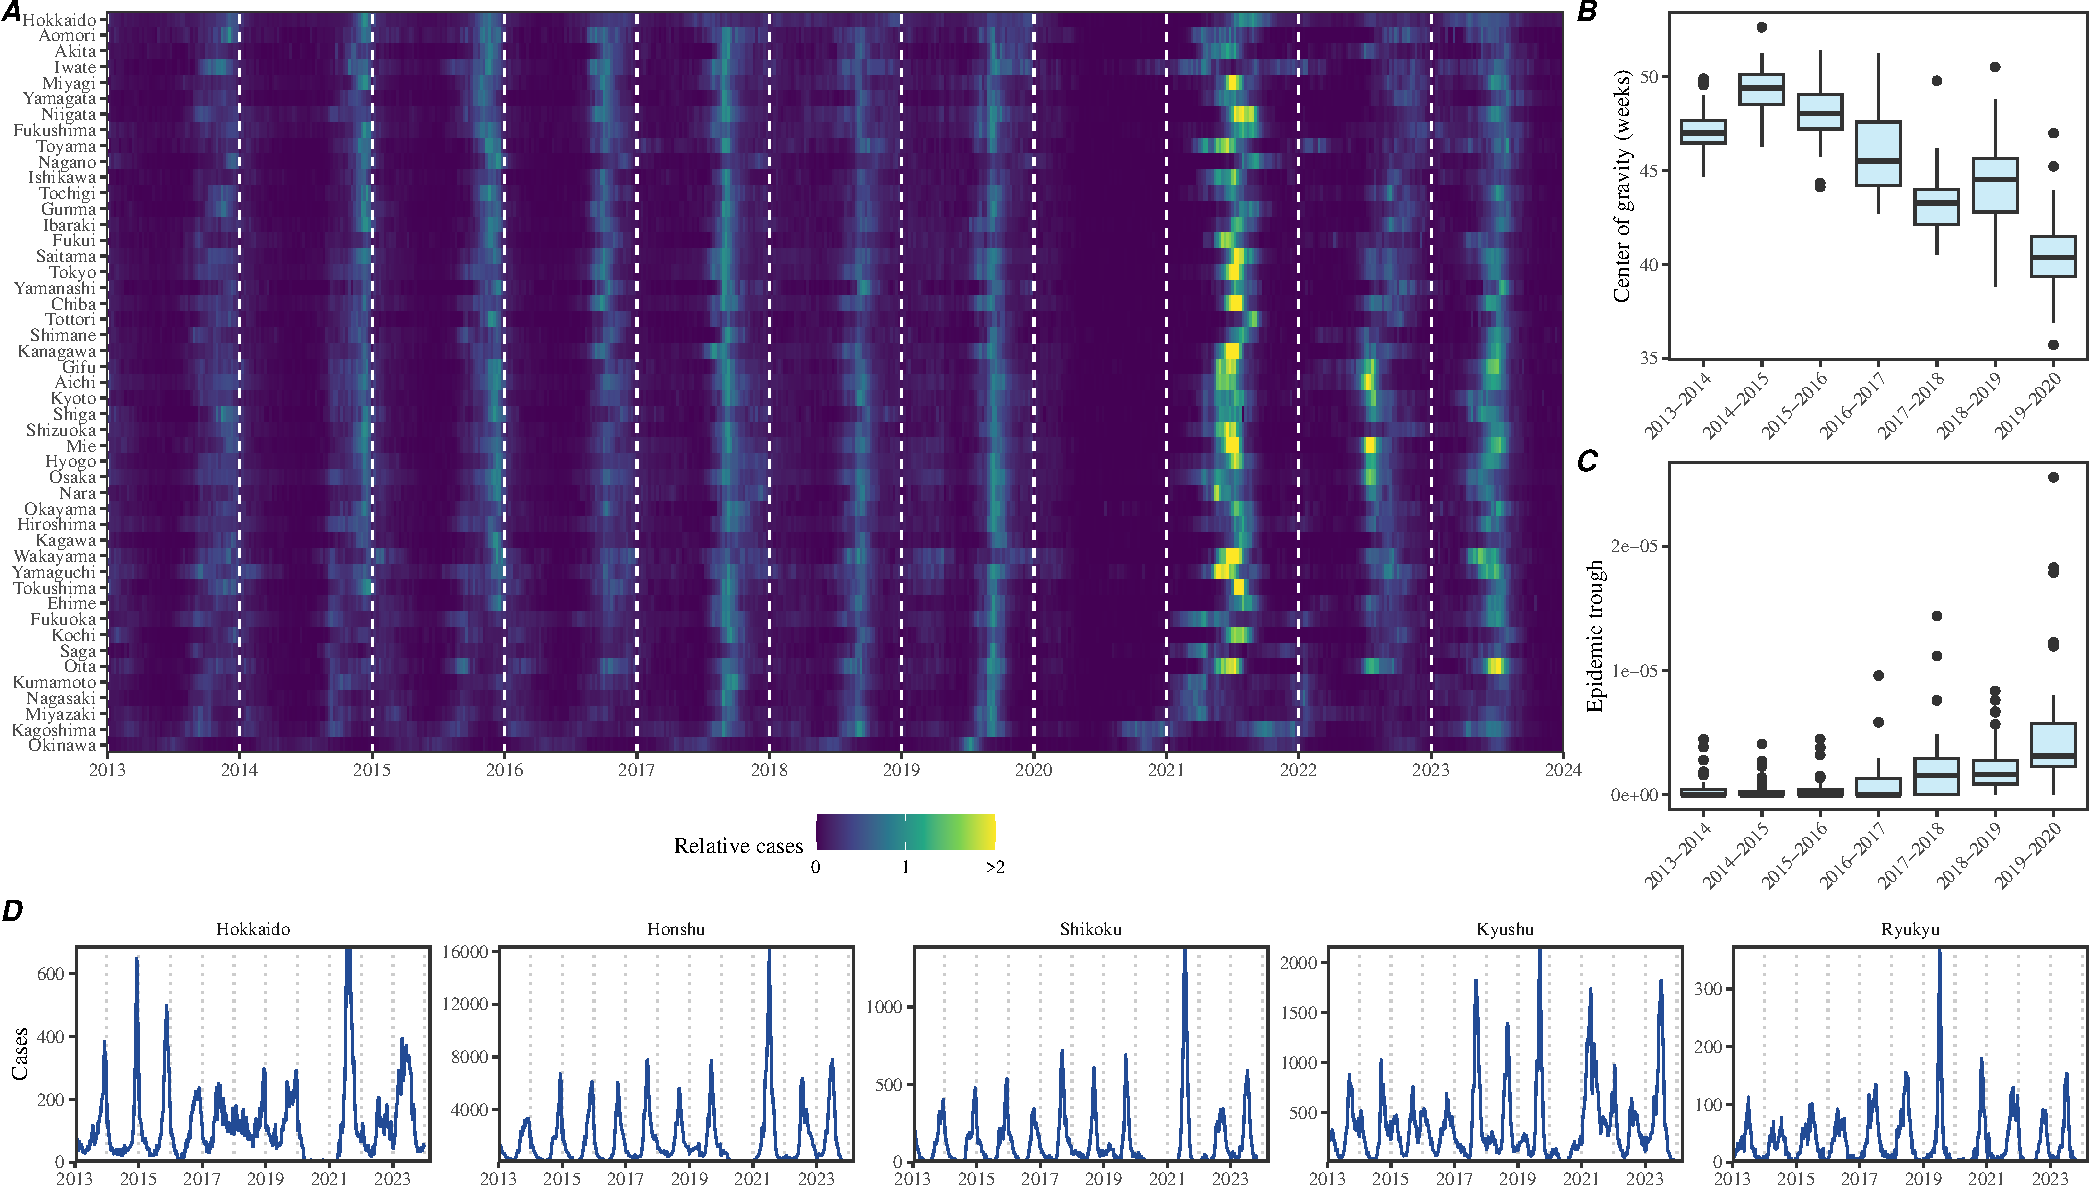
\includegraphics[width=\textwidth]{../figure/figure1.pdf}
\caption{
\textbf{Observed changes in RSV outbreak dynamics in Japan.}
(A) Relative RSV cases across 47 prefectures in Japan between 2013 and 2024.
Relative cases are calculated by dividing the raw cases by the pre-pandemic maximum.
(B) Estimates of center of gravity (i.e., the mean timing of an epidemic) across 46 prefectures, excluding Okinawa.
(C) Estimates of epidemic trough (i.e., the minimum number of cases in a season divided by the population size) across 47 prefectures.
(D) Time series of RSV cases across 5 major islands.
}
\label{fig:fig1}
\end{figure}

A sudden change in RSV seasonality from winter to fall outbreaks was observed in nearly all prefectures between 2016 and 2017 (\fref{fig1}A).
To quantify changes in seasonality, we calculated the center of gravity (i.e., the mean timing of an epidemic) for each outbreak season at every prefecture and found a conssitent decrease in the center of gravity (\fref{fig1}B; Methods). 
We also found that these changes were associated with an increase in epidemic troughs (\fref{fig1}C).

We found considerable heterogeneity in the observed outbreak dynamics across major islands, especially following the changes in seasonality (\fref{fig1}D).
For example, annual RSV outbreaks in Hokkaido island became more persistent, causing high numbers of cases throughout the year.
Semiannual RSV outbreaks in Shikoku and Kyushu islands became more annual and explosive, leading to sharper epidemics.
Finally, in contrast to all other islands, RSV outbreaks in Ryukyu island exhibited summer outbreaks, which in turn became more explosive leading up to 2020.

\subsection*{A parsimonious model for RSV epidemics}

We first began by asking whether a simple Susceptible-Infected-Recovered-Susceptible (SIRS) model can capture the observed RSV outbreak dynamics in Japan, especially the changes in seasonality.
The SIRS model is the simplest model that allows for waning of immunity and therefore represents one of the most parsimonious models for explaining outbreak dynamics of respiratory infections.
Here, we extended the standard SIRS model such that we could simultaneously estimate periodic seasonal transmission rates and changes in transmission due to non-pharmaceutical intervention (NPI) measures that were implemented to prevent COVID-19 (Methods).

\begin{figure}[!th]
\includegraphics[width=\textwidth]{../figure/figure_comb_sirs_npi.pdf}
\caption{
\textbf{Summary of SIRS model fits to RSV outbreaks across major islands in Japan.}
(A) Comparisons of observed cases (points) across five major islands and fitted epidemic trajectories (red lines).
(B) Estimated periodic seasonal transmission rates.
(C) Relationship between the estimated periodic seasonal transmission rates and mean specific humidity.
Points represent the estimates across 52 weeks.
Lines represent the corresponding locally estimated scatterplot smoothing (LOESS) estimates.
(D) Estimated relative changes in transmission, capturing the impact of NPI measures.
(E) Estimated proportion of the susceptible pool.
Lines represent the estimated median of the posterior distribution.
Shaded regions represent the 95\% credible intervals from the posterior distribution.
}
\label{fig:fig2}
\end{figure}

The SIRS model was able to reproduce the observed dynamics across all five islands, including changes in seasonality that occurred during 2016--2017 as well as post-pandemic changes in outbreak patterns (\fref{fig2}A).
Interestingly, we estimated semiannual peaks in transmission rates across all islands, except for the Hokkaido island (\fref{fig2}B).
These semiannual patterns in transmission were explained by the nonlinear effects of specific humidity;
we estimated that transmission would peak at low and high specific humidity (\fref{fig2}C).

Across all five islands, we estimated a considerable reduction in transmission during 2020  (\fref{fig2}D);
however, there were large heterogeneity in the overall shape of the estimated NPI effects as well as the degree of transmission reduction.
The reduction in transmission rates caused an increased in susceptibile pool (\fref{fig2E}), which allowed a large outbreak when NPIs were lifted (\fref{fig2}A).

\subsection*{Mechanisms for sudden changes in seasonality}

Since our SIRS model could accurately capture the observed dynamics, we were able to use our fits to further tease apart the mechanisms underlying sudden changes in seasonality of the RSV outbreaks.
To do so, we first began by evaluated the changes in the proportion of susceptible and infected individuals at the beginning of the season between 2013 and 2019;
we focused on three main islands that exhibited clear changes in seasonality: Honshu, Shikoku, and Kyushu islands. 

We found a consistent increase in the proportion of susceptible and infected individuals at the beginning of each season between 2013 and 2019 across three main islands (\fref{fig3}A).
These changes also corresponded with a decrease in center of gravity (\fref{fig3}A).
A more detailed comparison of epidemic trajectories illustrated that an increase in the susceptible pool at the beginning of season can drive a sudden shift in seasonality (\fref{fig3}B).

We also found considerable heterogeneity across islands in differences in peak epidemic timing associated with changes in seasonality (\fref{fig3}B): 9--12 weeks (Honshu), 6--11 weeks (Shikoku), and 18--20 weeks (Kyushu).
This heterogeneity can be explained by the differences in the seasonal transmission patterns (\fref{fig3}C--G).
Specifically, RSV transmsission in Honshu island (\fref{fig}3C) exhibits a narrower amplitude (\fref{fig3}D) and a narrower trough (\fref{fig3}E) compared to RSV transmission in Honshu island (\fref{fig3}E).
Simulating the SIRS model using seasonal transmission rates that interpolate those estimated from two islands confirmed that a large seasonal amplitude and wider trough cause larger changes in the timing of epidemic peak (\fref{fig3}F). 

\begin{figure}[!th]
\includegraphics[width=\textwidth]{../figure/figure_comb_sirs_change.pdf}
\caption{
\textbf{An increase in the susceptible pool explains sudden changes in seasonality.}
(A) Predicted effects of the proportion of infected $I(0)$ and susceptible $S(0)$ at the beginning of season on center of gravity.
Points represent the observed values for $I(0)$ and $S(0)$ between 2013 and 2019.
(B) Changes in epidemic trajectories caused by an increase in the susceptible proportion at the beginning of season from 7.8\% to 10.5\%.
(C--F) Comparisons of interpolated transmission rates used for simulating the SIRS model, corresponding to each corner in Panel G. 
Black lines represent the transmission rates used for simulations. 
Gray lines represent the estimated transmission rates the Honshu island as a visual reference.
(C) The estimated transmission rates for the Honshu island.
(D) The resulting transmission rates for the Honshu island when we increase the amplitude to match the amplitude of the transmission rates for the Kyushu island.
(E) The resulting transmission rates for the Kyushu island when we decrease the amplitude to match the amplitude of the transmission rates for the Honshu island.
(F) The estimated transmission rates for the Kyushu island.
(G) Differences in peak epidemic timing when we increase the the susceptible proportion at the beginning of season from 7.8\% to 10.5\% across different assumptions about the underlying transmission rate. 
}
\label{fig:fig3}
\end{figure}

\subsection*{Mechanisms for an increase in population-level susceptibility}

So what mechanisms caused the population-level susceptibility to increase over time in Japan?
We hypothesized that the Comprehensive Support System for Children and Childcare, which was enacted in 2012 and launched in 2015, contributed to an increase in the population-level susceptibility:
specifically, an expansion of childcare facilities would increase contact rates among children, effectively, increasing their susceptibility.
To quantify the effect of this program, we compared the number of children attending childcare facilities in Japan since 2013 and compared them with our estimates of susceptible proportion (\fref{fig4}).
Overall, we found consistent patterns of increase in childcare attendance and strong correlations with the estimated susceptible proportion: 

\begin{figure}[!th]
\includegraphics[width=\textwidth]{../figure/figure_childcare.pdf}
\caption{
\textbf{Increase in the susceptible pool following the launch of the Comprehensive Support System for Children and Childcare in Japan.}
(A) Direct comparisons between the estimates of susceptible proportion at the beginning of each season in each island (black) and the number of children attending childcare facilities in Japan (red).
Shaded regions represent the 95\% credible interval in our estimates.
(B) Correlations between the estimates of susceptible proportion at the beginning of each season in each island and the number of children attending childcare facilities in Japan.
Error bars represent  the 95\% credible interval in our estimates.
Red lines and shaded regions represent the best fitting linear regression and the corresponding 95\% confidence intervals.
}
\label{fig:fig4}
\end{figure}

\section*{Discussion}

We present an epidemiological analysis of RSV outbreaks in the Japan using mathematical modeling approach.
Our analysis revealed semiannual cycles in seasonal RSV transmission, which correlate with specific humidity.
We found that these semiannual cycles allowed a sudden shift in the seasonality of RSV outbreaks through an increase in population-level susceptibility.
We tentatively hypothesize that an increase in childcare capacity in Japan may be a main driver of the increase in  population-level susceptibility.



\section*{Methods}

\pagebreak

\bibliography{perturbation}

\end{document}
